\begin{surferPage}{Eine $A_4^{++}$ Singularität}
Genauso wie die $A_4^{+-}$ Singularität der $A_2^{+-}$ Singularität vom
    Aussehen her sehr
    ähnelt, ist es mit der $A_4^{++}$ und der $A_2^{++}$ Singularität. 
    Hier die Bilder in der Reihenfolge
    $A_2^{++}$, $A_4^{++}$,$A_2^{+-}$, $A_4^{+-}$:
    \begin{center}
      \vspace*{-0.2cm}
      \begin{tabular}{@{}c@{\ }c@{\ }c@{\ }c@{}}
        \begin{tabular}{@{}c@{}}
          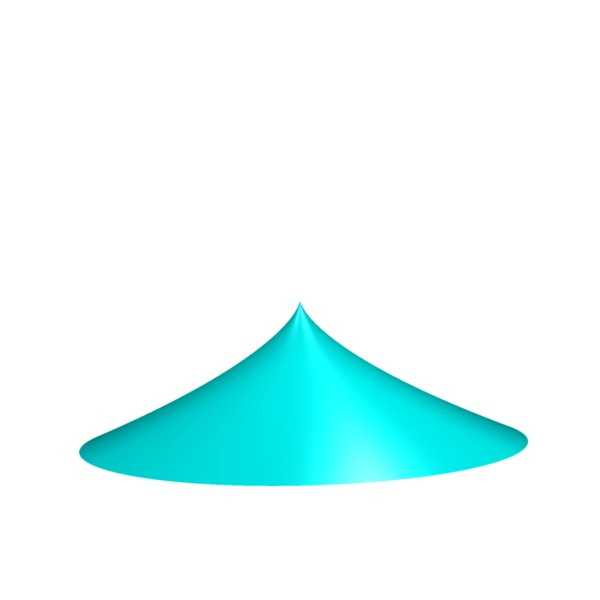
\includegraphics[width=1.2cm]{../../common/images/A2pp}
        \end{tabular}
        &
        \begin{tabular}{@{}c@{}}
          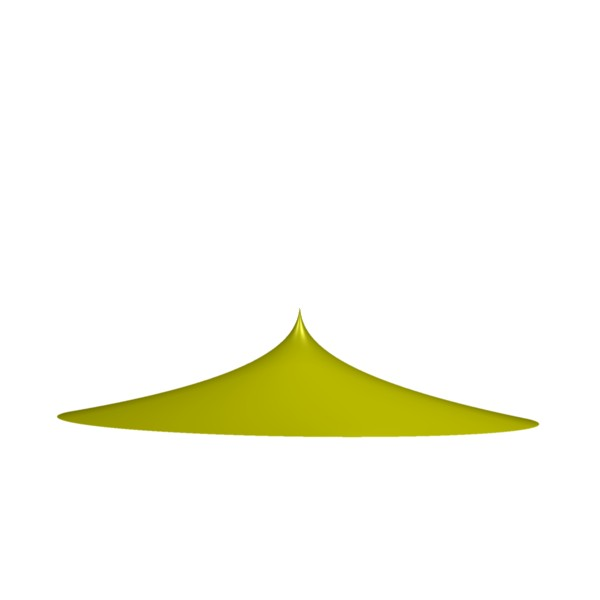
\includegraphics[width=1.2cm]{../../common/images/A4pp}
        \end{tabular}
        &
        \begin{tabular}{@{}c@{}}
          
\includegraphics[width=1.2cm]{../../common/images/A2pm}
        \end{tabular}
        &
        \begin{tabular}{@{}c@{}}
          
\includegraphics[width=1.2cm]{../../common/images/A4pm}
        \end{tabular}
      \end{tabular}
    \end{center}
    \vspace*{-0.2cm}
    Jeweils lässt sich bei den Singularitäten vom Typ $A_4$ erkennen, dass sie
    ``steiler'' auf den singulären Punkt zulaufen.

    Wie auch schon bei der $A_4^{+-}$ Singularität offenbart sich der große
    Unterschied zwischen $A_4$ und $A_2$ erst bei genauerem Hinschauen; z.B.\
    beim Versuch, die Singularität in möglichst viele Doppelkegel zu
    deformieren: 
    Die $A_2^{++}$ Singularität lässt sich nur in einen, die $A_4^{++}$ Singularität
    aber in zwei Doppelkegel deformieren:
%    \dontshow{
    % 
    \begin{center}
      \vspace*{-0.2cm}
      \begin{tabular}{@{}c@{\quad}c@{\quad}c@{}}
        \begin{tabular}{@{}c@{}}
          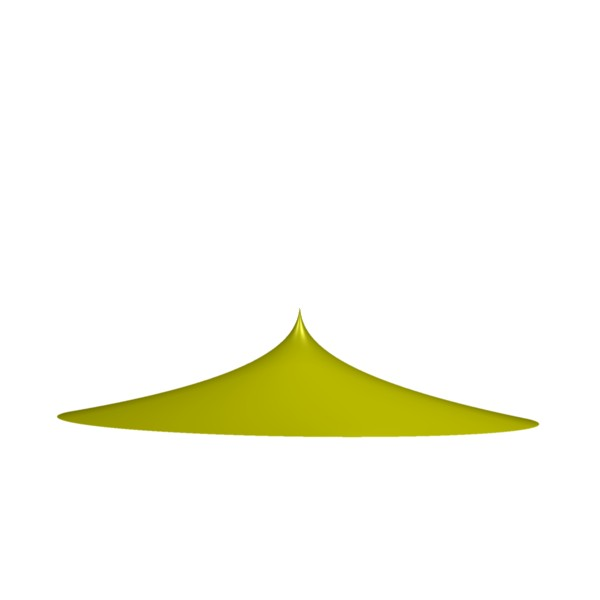
\includegraphics[width=1.2cm]{../../common/images/A4pp_0}
        \end{tabular}
        &
        \begin{tabular}{@{}c@{}}
          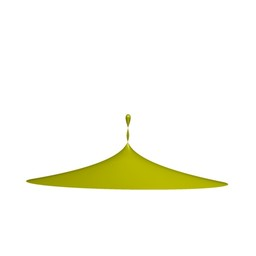
\includegraphics[width=1.2cm]{../../common/images/A4pp_1}
        \end{tabular}
        &
        \begin{tabular}{@{}c@{}}
          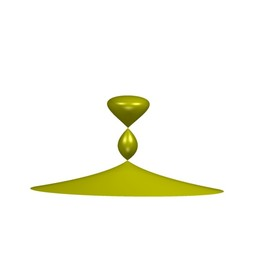
\includegraphics[width=1.2cm]{../../common/images/A4pp_2}
        \end{tabular}
      \end{tabular}
    \end{center}
%    }
      \vspace*{-0.2cm}
    Dies realisiert die Gleichung:
    \[x^2(x+a^2)^2(x-a^2)+y^2+z^2.\]
 
\end{surferPage}
